\documentclass{article}

% Language setting
% Replace `english' with e.g. `spanish' to change the document language
\usepackage[spanish]{babel}

% Set page size and margins
% Replace `letterpaper' with `a4paper' for UK/EU standard size
\usepackage[a4paper,top=2cm,bottom=2cm,left=3cm,right=3cm,marginparwidth=2cm]{geometry}

% Useful packages
\usepackage{amsmath}
\usepackage{graphicx}
\usepackage[colorlinks=true, allcolors=black]{hyperref}
\usepackage{fancybox}
\usepackage{listings}
\usepackage{subcaption}
%\lstset{
%    language=Matlab,
%    extendedchars=true
%}

\title{Comportamiento del protocolo Aloha Ranurado}
\author{Álvaro Hernández Riquelme}
%\date{}

\begin{document}
\maketitle

\tableofcontents
\newpage

%\begin{abstract}
%Your abstract.
%\end{abstract}


\section{Introducción al trabajo}

Para este trabajo, se estudiará el comportamiento de un protocolo de Aloha Ranurado usando un sistema SDL, donde se completará la edición, simulación y validación total del protocolo. Tras esto, se hará un estudio de éste.

\quad

\textbf{SDL}, también conocido como Simulation and Description Language, es el lenguaje de especificación formal creado por la ITU para definir y representar sistemas y protocolos. Se usará la herramienta \textbf{Telelogic Tau}, para representar nuestra especificación de \textbf{Aloha Ranurado}. Tendremos una base sin terminar del protocolo en el aula virtual, la cual modificaremos y completaremos, finalmente haremos una simulación y validación. 

\quad

\textbf{Aloha} es un protocolo de acceso al medio aleatorio, donde varios nodos pueden compartir información con una probabilidad de colisión, ya que se envía la información sin comprobar si el canal está libre. Quiere decir que si en el tiempo de envío, existe otro nodo transmitiendo, se producirá ésta colisión. Para mejorar las prestaciones, se define \textbf{ALOHA ranurado}, donde se dividen las transmisiones de mensajes en slots del tamaño de éste mensaje y los nodos solo pueden transmitir al inicio de los slots. De este modo, se reduce el periodo de colisión.

\subsection{Nuestro Entorno}

Como se ha dicho previamente, usaremos Telelogic Tau para la simulación del protocolo. Al abrirlo, si cargamos la base del trabajo proporcionada en el aula virtual, podremos empezar a trabajar sobre ésta.

\quad

\begin{figure}[h]
    \centering
    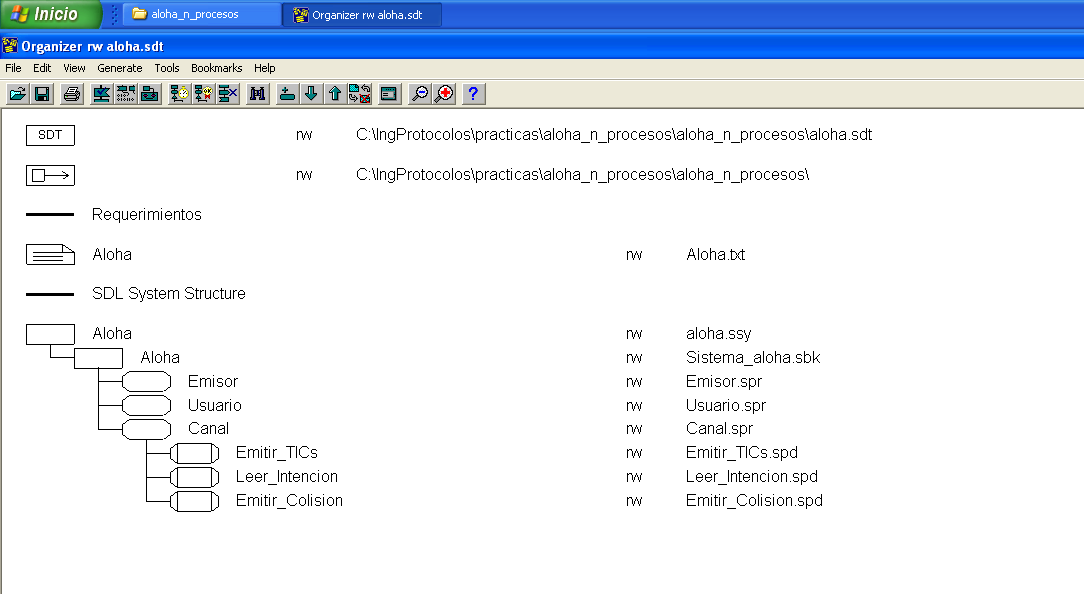
\includegraphics[width=1\linewidth]{src/Organizer-tltau.png}
    \caption{\label{fig:tltau} Inicio de Telelogic Tau con el proyecto de ALOHA Ranurado.}
\end{figure}

\newpage

\section{Edición}

Como se nos ha comentado en clase, antes de ir a la simulación y validación, tendremos que emepzar con la edición, ya que la base proporcionada no está completa. Teniendo en cuenta la captura anterior, y usando el programa para ver qué hay hecho, vemos que los procesos \textbf{Emisor, Usuario, y Canal} están sin terminar, por lo que empezaremos diseñando estos estados.
Es importante reconocer qué significa cada símbolo:

\begin{figure}[h]
    \centering
    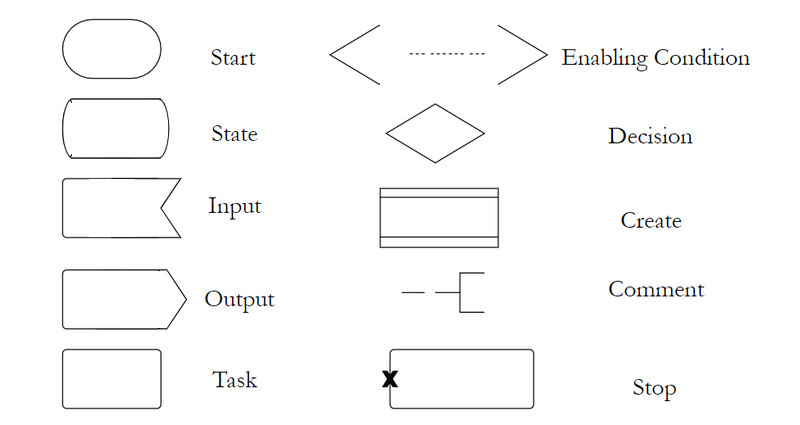
\includegraphics[width=0.7\linewidth]{src/sdl-symbols.jpg}
    \caption{\label{fig:sdlsymbols} Significado de los símbolos en SDL.}
\end{figure}

\quad

\subsection{Emisor}

Para el bloque \textbf{emisor}, crea su correspondiente instancia de proceso usuario, entonces le damos a user el valor de \verb|Offspring|,  que es una variable del sistema que nos permitirá asignar una ID a cada usuario. Una vez esto, el usuario puede que tenga un mensaje que transmitir o no. Dependiendo irá por una rama o por otra. 

\begin{figure}[h]
    \centering
    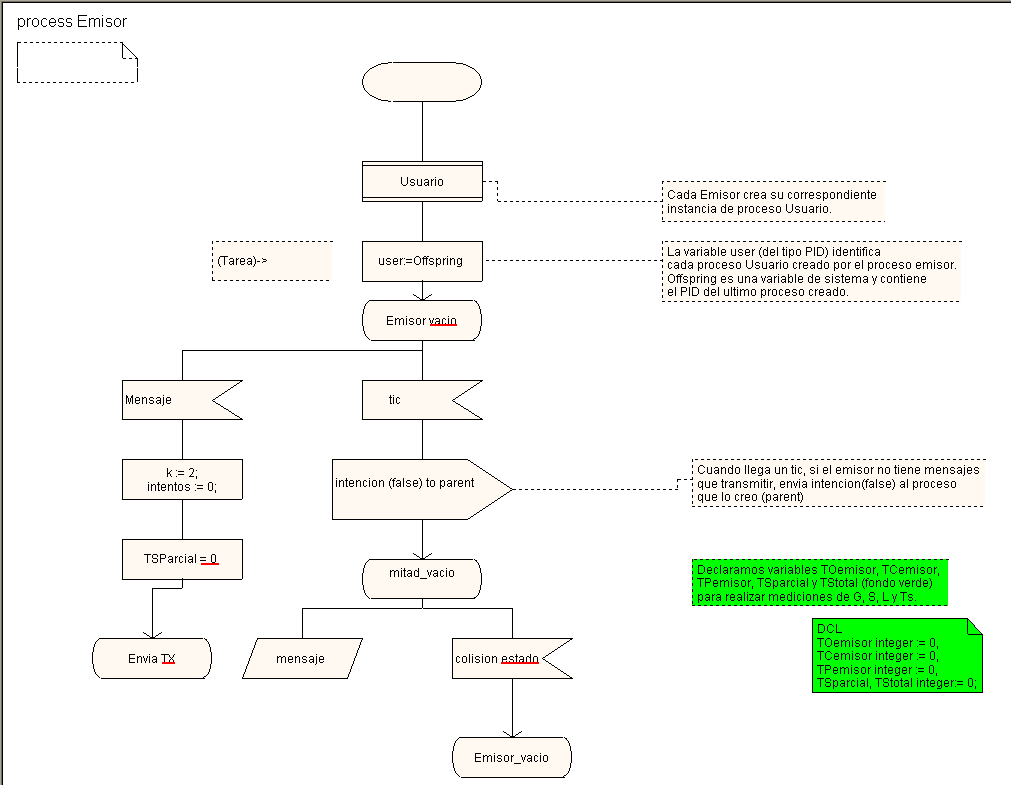
\includegraphics[width=0.8\linewidth]{src/Estado emisor.png}
    \caption{\label{fig:emisorbl} Diagrama del estado/proceso emisor.}
\end{figure}

Vemos que al iniciar el emisor, en el momento que llega a \verb|Emisor vacío|, espera 2 tipos de inputs: mensaje o tic. En caso de que haya un mensaje que transmitir, va a la izquierda, donde asignamos una k y reseteamos los intentos para transmisión y el tráfico parcial. Iríamos al estado \verb|Envía TX|. En cambio, si no hay un mensaje que transmitir, recibiríamos un tic, donde se envía la intención de que efectivamente no queremos transmitir a quien lo creó y, en caso de que haya un mensaje para transmitir se guardaría para el siguiente tic y si no, iríamos de vuelta al estado \verb|Emisor vacío|. 

\subsubsection{Estado Envia TX}

El estado empieza esperando a recibir el input del próximo tic, al pasar, aumentaremos en 1 las variables de TOemisor y TSparcial. En este caso, en vez de enviar la intención de que \textbf{no} queremos envíar, envíamos que \textbf{sí} querríamos, con un true. Al entrar al estado \verb|ficticio|, comprobamos con el input de estado, si existe colisión o no, por lo que si no hubiera, el proceso \verb|Emisor| crearía un \verb|Usuario| (envía true a usuario). en caso contrario, se aplicaría el algoritmo backoff un número máximo de reintentos como mucho, siendo que si no lo conseguimos finalmente, no se enviaría el resultado true a \verb|Usuario|.
Vemos el diagrama de \verb|Envía TX|:

\quad

\begin{figure}[h]
    \centering
    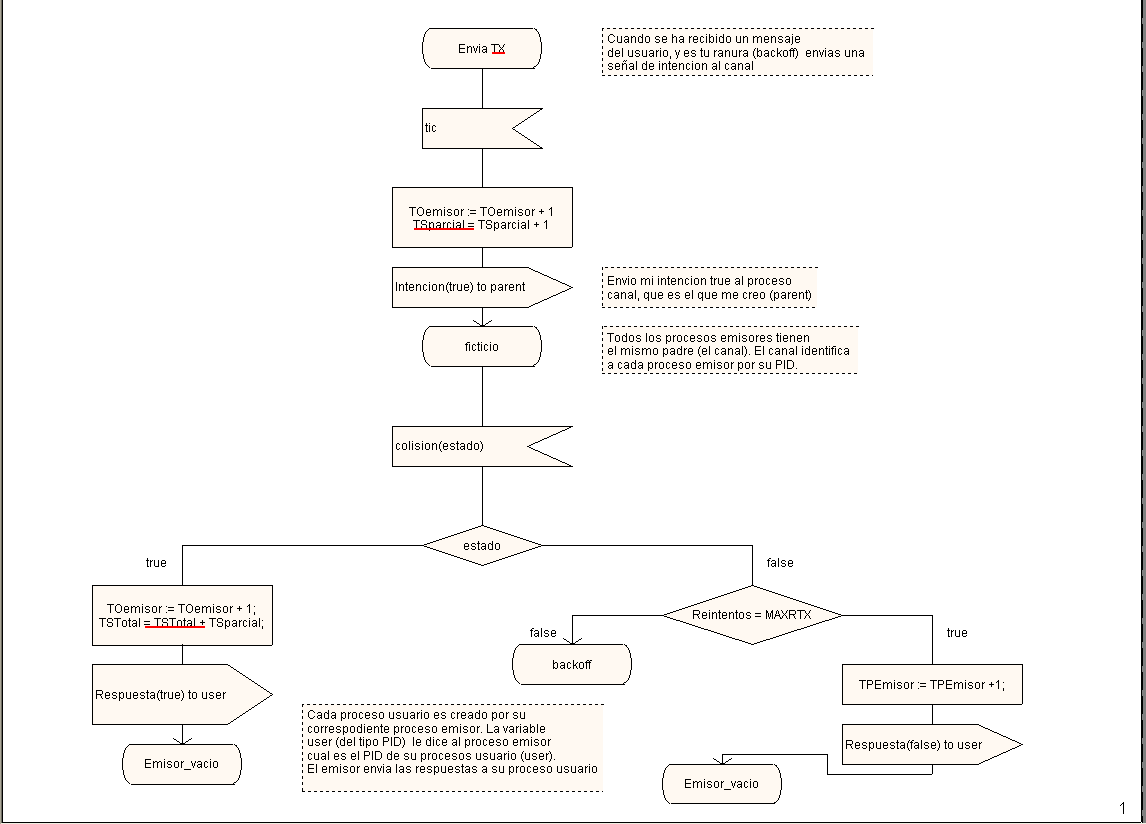
\includegraphics[width=0.8\linewidth]{src/Estado enviatx.png}
    \caption{\label{fig:enviatxbl} Diagrama del estado Envia TX.}
\end{figure}



\subsubsection{Algoritmo Backoff}

Como hemos visto antes, es posible que en el estado haya una colisión al intentar transmitir el mensaje, es por eso que si el estado de colisión nos devuelve \textbf{false}, y no nos hemos pasado el límite de intentos, iremos al algoritmo \verb|backoff|.

En este estado, simplemente generaremos un número aleatorio \textbf{k} de ranuras, y las iremos reduciendo en cada tic hasta llegar a 0, donde llegaría el turno de enviar otra vez, e intentaríamos de nuevo enviar volviendo al estado \verb|Envía TX|, podría ser que se envíe tras el estado, o que vuelva a haber colisión, se generaría un bucle hasta que no haya colisión o no supere el máximo de intentos.
\newpage

\begin{figure}[htb]
    \centering
    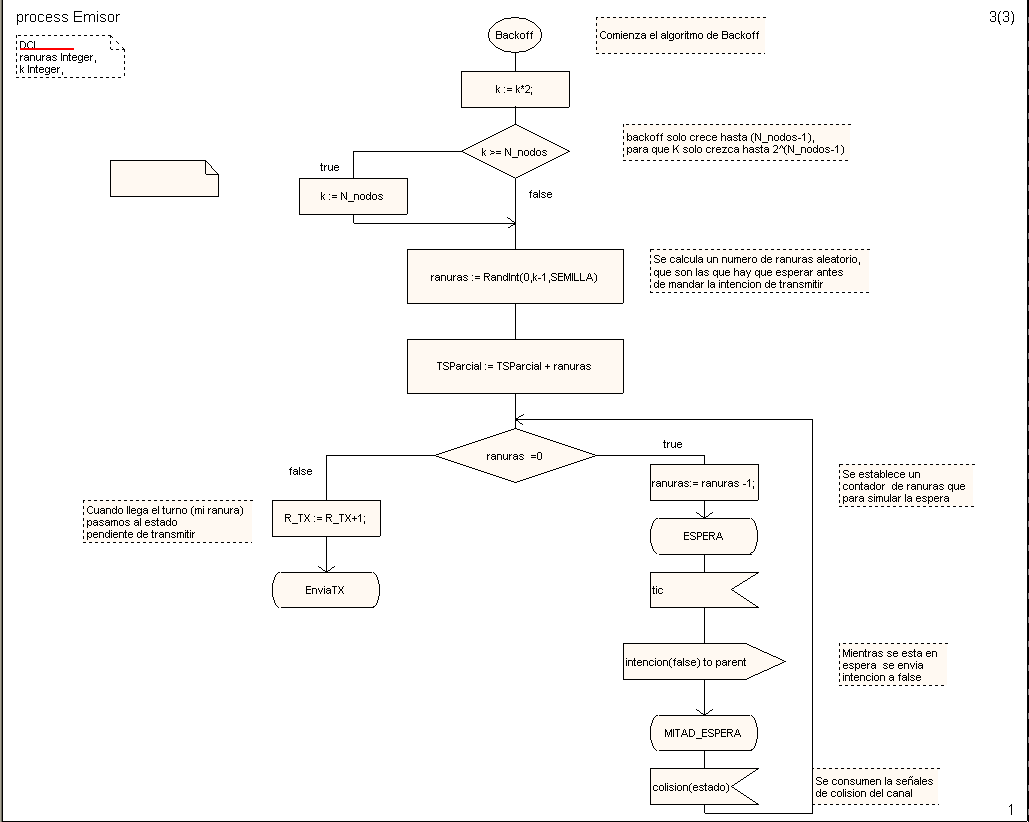
\includegraphics[width=0.85\linewidth]{src/backoff state.png}
    \caption{\label{fig:backoffstate} Diagrama del Algoritmo Backoff.}
\end{figure}

\quad

\subsection{Usuario}

El proceso usuario nos indicará si existe una intención de transmitir o no. Será el encargado de enviárselo al emisor. Consistirá en una probabilidad Pg donde puede \textbf{enviarse o no. (true o false)}

\quad

\begin{figure}[h]
    \centering
    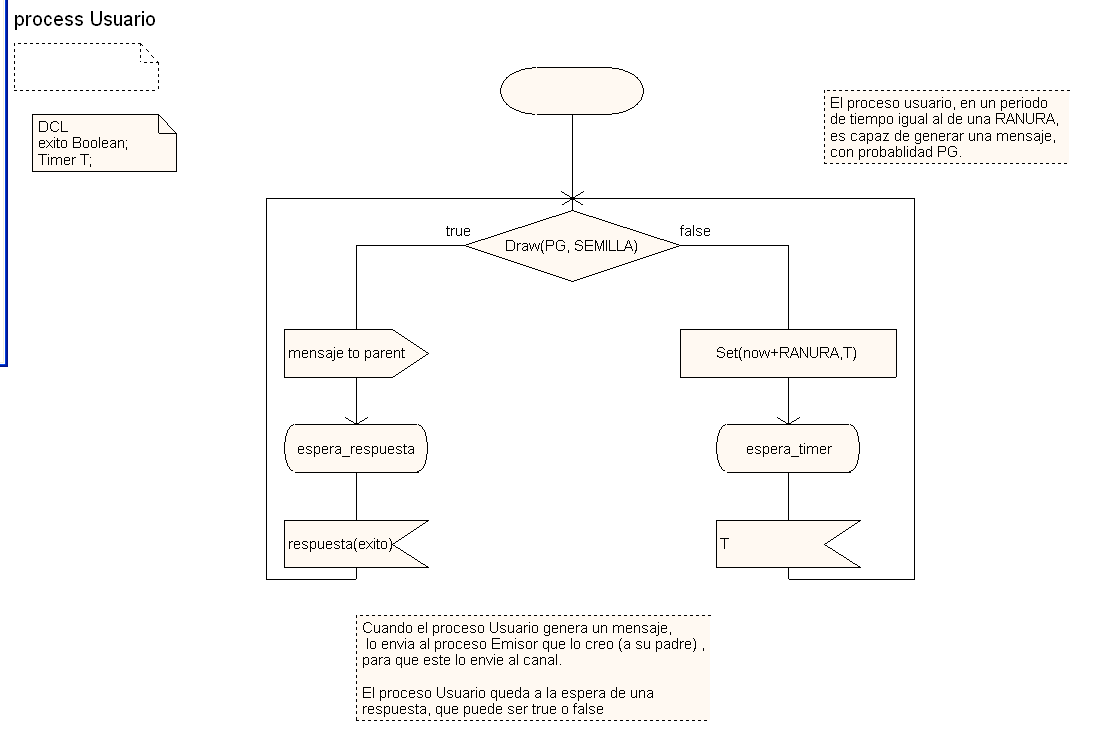
\includegraphics[width=0.7\linewidth]{src/captura usuario.png}
    \caption{\label{fig:usuariodiagr} Diagrama del proceso Usuario.}
\end{figure}

\quad

Cabe destacar que, tal como nos indicaba el manual sobre ALOHA, debíamos insertar la función set, teniendo como parámetro de "\(\)Expr " \textbf{RANURAS}, y de "TimerName" \textbf{T}. \textbf{PREGUNTAR NO PUEDO EDITAR}

\subsection{Canal}

El canal se encarga de mantener la estabilidad y organización del sistema, esto es, debido a que lleva el conteo de tics (Como si fuera el clk) y a la vez con los procedimientos \verb|Leer intención| y \verb|Emitir colisión| comprobaremos si existe colisión y se lo comunicaremos a los demás procesos.

\quad

Entonces, finalmente en la captura veremos que este proceso termina en un "bucle" donde generamos un tic, y según las intenciones emitiremos una colisión o no:

\begin{figure}[h]
    \centering
    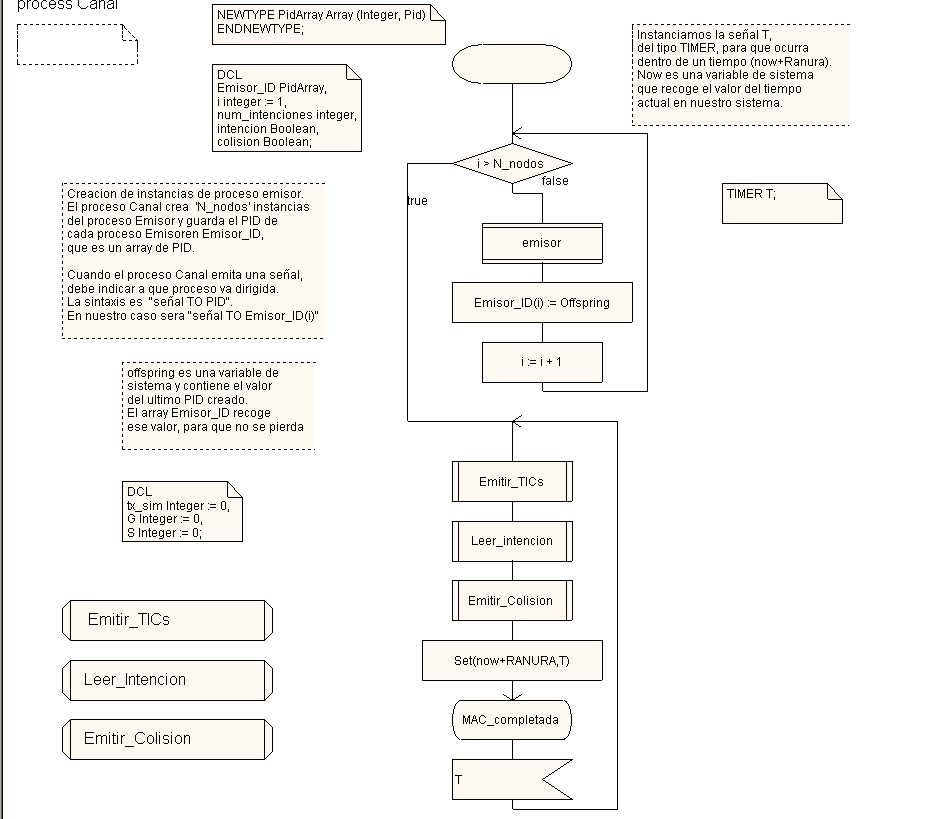
\includegraphics[width=0.8\linewidth]{src/proceso canal.png}
    \caption{\label{fig:canalproceso} Diagrama del proceso del canal.}
\end{figure}


En el proceso de canal, tendremos tres procedimientos: \textbf{emitir tics}, \textbf{leer intención}, y \textbf{emitir colisión}:

\subsubsection{Emitir Tics}

Éste procedimiento, únicamente lo que hará será tener un contador que será  incrementado cada vez que se le llama, y a la vez se lo enviará como Output al \verb|Emisor| , como vemos en \textbf{tic to Emisor id i}

\begin{figure}[hbt]
    \centering
    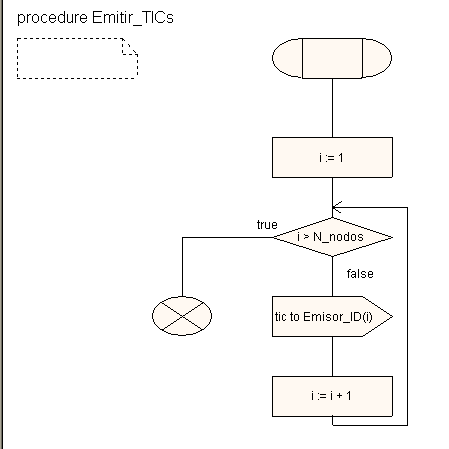
\includegraphics[width=0.3\linewidth]{src/proc emitir tics.png}
    \caption{\label{fig:emitirtics} Procedimiento emitir tics.}
\end{figure}

\subsubsection{Leer Intención}

El procedimiento leer intención, recibirá el input de intención, y dependiendo de si hay intención o no, (true o false), se incrementará la variable numi o i.

\quad

\begin{figure}[h]
    \centering
    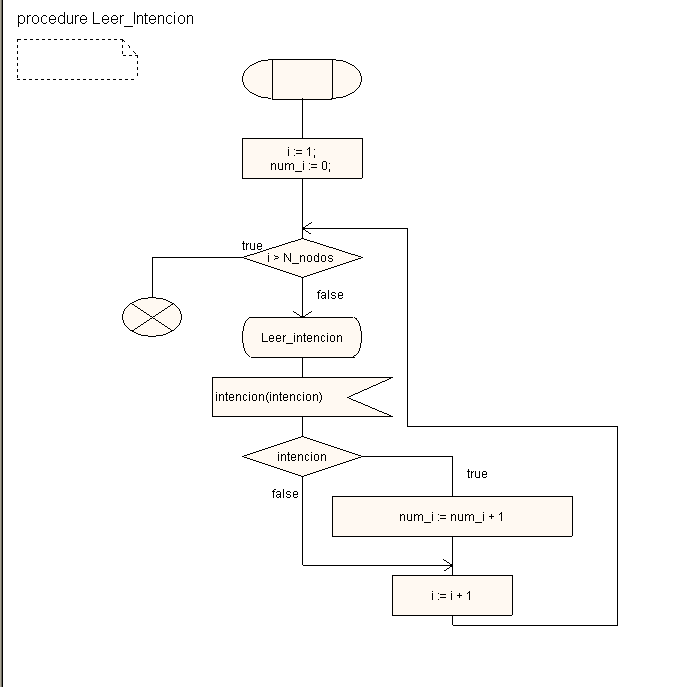
\includegraphics[width=0.6\linewidth]{src/leer intencion.png}
    \caption{\label{fig:leerintencion} Procedimiento leer intencion.}
\end{figure}

\subsubsection{Emitir colisión}

En el procedimiento de leer intención hemos visto, que si hay intención de transmitir, incrementaremos 1 en la variable numi. En este caso, en emitir colisión, usaremos esta variable para confirmar si existe o no una colisión, y emitirla en caso afirmativo. Ésto pasaría, cuando la variable numi es mayor que uno (Más de una intención de transmitir en el canal), en este caso pondríamos colisión en \textbf{True.}

\quad

\begin{figure}[h]
    \centering
    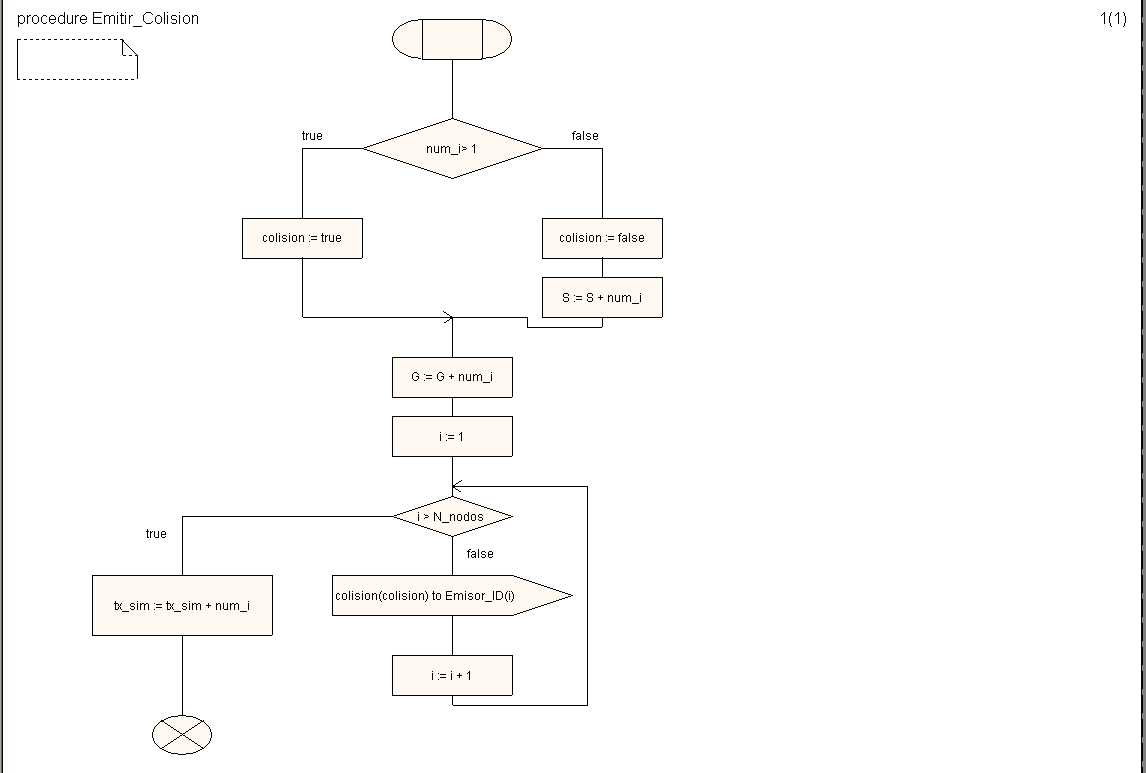
\includegraphics[width=0.8\linewidth]{src/proc emitir col.png}
    \caption{\label{fig:emitircol} Procedimiento emitir colisión.}
\end{figure}
\newpage

\section{Validación}


\end{document}